\documentclass{beamer}
\usepackage{HECbeamer}
\usepackage{icomma}
\newcommand{\AIC}{\textsf{AIC}}
\newcommand{\BIC}{\textsf{BIC}}
% \usepackage{pgfpages}
% \pgfpagesuselayout{4 on 1}[letterpaper, landscape, border shrink=5mm]
\title[\color{white}{MATH 60604 \S~4h - Modèle binomiale et proportions}]{\texorpdfstring{MATH 60604 \\Modélisation statistique \\ \S~4h - Modèle binomiale et proportions}{MATH 60604 \\Modélisation statistique \\ \S~4h - Modèle binomiale et proportions}}
\author{Léo Belzile}
\institute{HEC Montréal\\
Département de sciences de la décision}
\date{} 

\begin{document}
\frame{\titlepage}

\begin{frame}
 \frametitle{Régression logistique pour des proportions}
 
 \bi \item Souvent, seules les données aggrégées sont disponibles et on a accès au nombre de réussites (sur $m$ essais).
 \item On peut utiliser la loi binomiale pour le modèle logistique en ajoutant le nombre d'essais au modèle.
 \item L'interprétation des paramètres reste identique.
 \ei 
 On considère le taux de succès dans 346 centres pour examens de conduite pratique en Grande-Bretagne; \href{https://www.gov.uk/government/statistical-data-sets/driving-test-statistics-drt}{les données sont pour 2018}.

\bi 
\item $761\ 750$ personnes on réussi l'examen pratique, pour $1\ 663\ 897$ essais.
\item \href{https://www.theguardian.com/world/2019/aug/23/an-easy-ride-scottish-village-fuels-debate-driving-test-pass-rates}{Un article du journal \textit{The Guardian} a suggéré que le taux de réussite était significativement plus élevé dans la campagne écossaise}. Puisque nous n'avons pas de classification des centres de test ruraux/urbains, on utilise le nombre d'examens passés comme proxy.
\item Les autres variables explicatives sont le \texttt{sexe} et la région en Angleterre; toutes les régions d'Écosse et du Pays de Galles sont regroupées.
\ei
 \end{frame}
 \begin{frame}
 \frametitle{Modèle binomial logistique pour examens de conduite britanniques}
 \begin{center}
  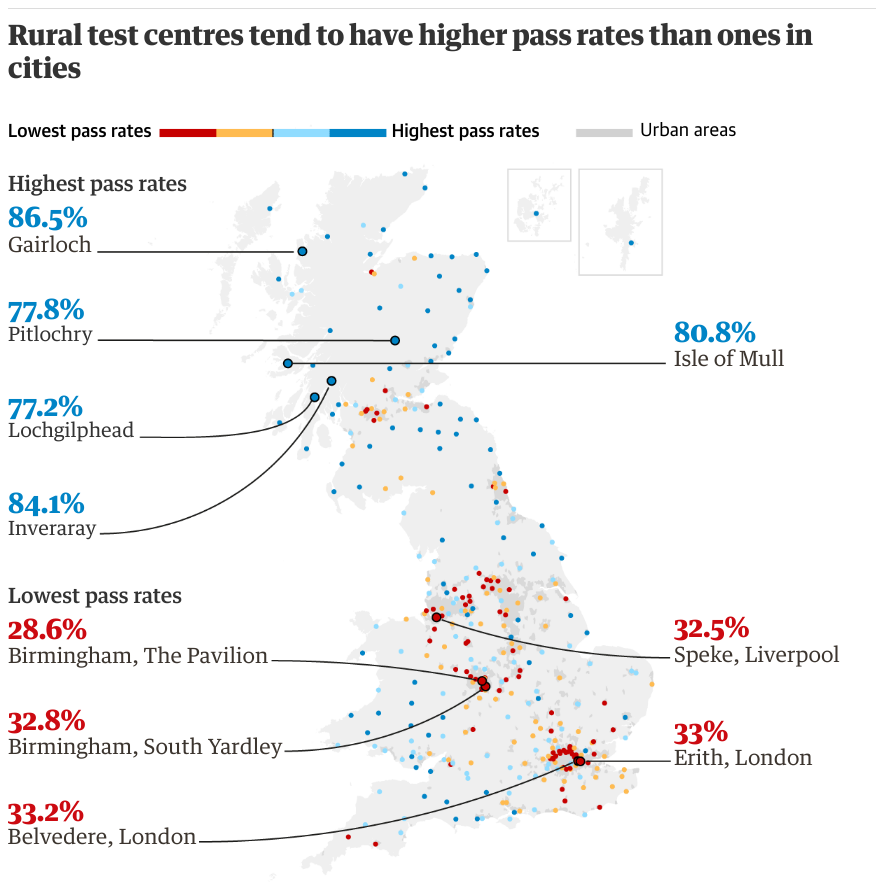
\includegraphics[width = 0.6\linewidth]{img/c4/01-intro-Guardian_UK_driving2.png}
 \end{center}
 {\footnotesize 
Source: \href{https://www.theguardian.com/world/2019/aug/23/an-easy-ride-scottish-village-fuels-debate-driving-test-pass-rates}{The Guardian}.}
\end{frame}
\begin{frame}[fragile]

\begin{tcolorbox}[colback=white, colframe=hecblue, title=Code SAS pour régression logistique binomiale]
\begin{verbatim}
data gbconduite;
set modstat.gbconduite;
if(total < 500) then volume="petit"; 
else if (total < 1000) then volume="moyen";
else volume = "grand";
run;

proc logistic data=gbconduite;
class sexe(ref="femme") region(ref="London")
    volume / param=glm;
model reussite/total = sexe region volume /
     plrl plcl expb;
run;
\end{verbatim}
\end{tcolorbox}
\end{frame}
\begin{frame}
 \frametitle{Taille des centres par région}
 \begin{center}
  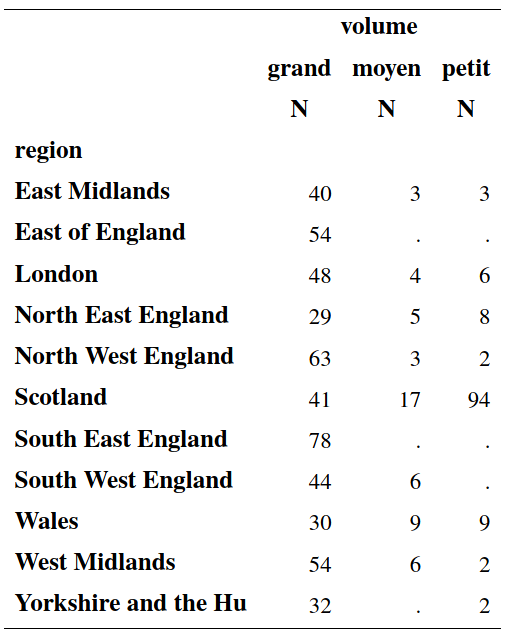
\includegraphics[width = 0.4\linewidth]{img/c4/diapos8-e23}
 \end{center}
{ \small La plupart des petits centres (moins de 500 examens par année) sont situés en Écosse.


}
\end{frame}

\begin{frame}
 \frametitle{Spécification du modèle}
 \begin{center}
 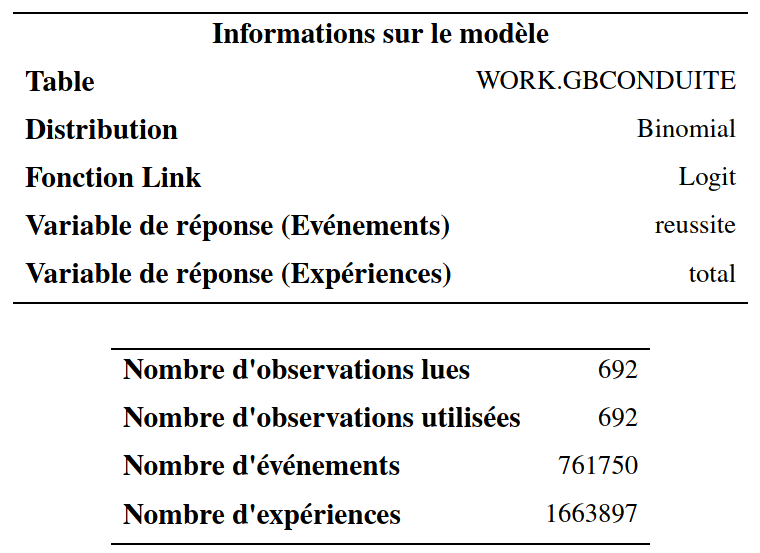
\includegraphics[width = 0.48\linewidth]{img/c4/diapos8-e19}
  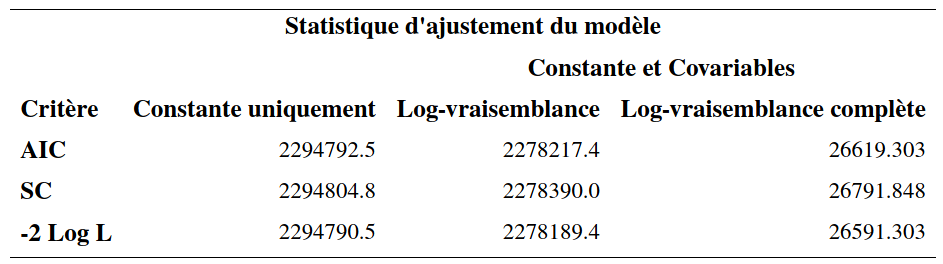
\includegraphics[width = 0.75\linewidth]{img/c4/diapos8-e20}
  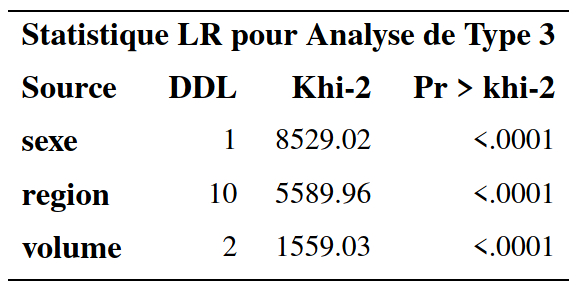
\includegraphics[width = 0.35\linewidth]{img/c4/diapos8-e21}
 \end{center}

\end{frame}

\begin{frame}
 \frametitle{Estimés des cotes pour les examens de conduite britanniques}
 \begin{center}
 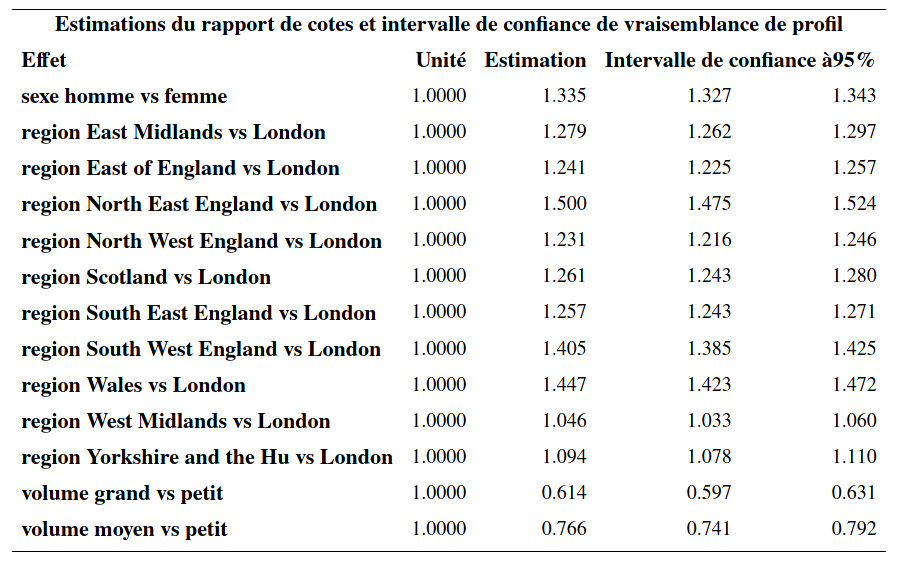
\includegraphics[width = 0.9\linewidth]{img/c4/diapos8-e22}
 \end{center}
\end{frame}

\begin{frame}
 \frametitle{Interprétation des paramètres pour les examens de conduite britanniques}
 Toute autre chose étant égale par ailleurs,
 \bi \item La cote des hommes pour la réussite de l'examen est $33\%$ plus élevée que celle des femmes;
 \item Londres est la région avec le plus faible taux de succès, même en prenant en compte le volume des centres de test; la cote pour la réussite est $50\%$ plus élevée en Angleterre du Nord-Est et $44.7\%$ plus élevée au Pays de Galles, etc.
  \item La cote du taux de réussite est $63\%$ plus grande dans les petits centres que dans les grands ($1/0.614$).
  \item Tous les paramètres sont statistiquement significatifs.
 \ei 
\end{frame}


\begin{frame}
 \frametitle{Remarque pour les modèles pour données binomiales/Bernoulli}
 \bi \item Si la déviance et la statistique du $X^2$ de Pearson sont parfois rapportées, leur loi nulle dépend des paramètres inconnus $\bs{\beta}$.
 \item Ainsi, la déviance ne suit qu'approximativement une loi $\chi^2_{n-p-1}$ et ce même quand le nombre d'essais $m$ est de l'ordre de plusieurs milliers.
 \item Les comparaisons de déviance entre modèle (ce qui revient à faire des tests de rapport de vraisemblance) sont néanmoins toujours valides.
  \ei
\end{frame}

\begin{frame}
 \frametitle{Accidents de la route aux États-Unis, prise deux}
 On peut ajuster un modèle binomial aux données \texttt{accident} où l'événement d'intérêt est le décès.
 
 \begin{center}
  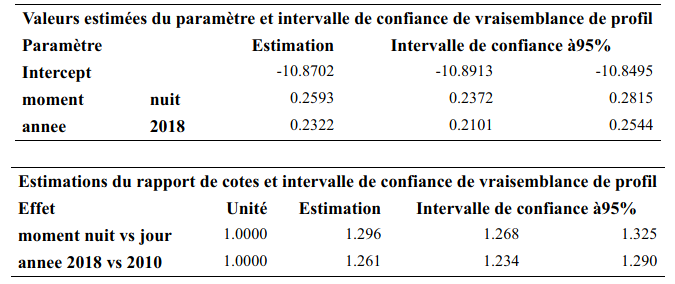
\includegraphics[width = 0.7\linewidth]{img/c4/diapos8-e24}
 \end{center}
 {\small
\bi \item Le taux estimé de décès sur la route le jour en 2010 est
$\hat{\pi}=\exp(\hat{\beta}_0)/\{1+\exp(\hat{\beta}_0)\} = 0,0000019016$, soit $1,9$ morts par $100 000$ habitants. Cet estimé du taux est légèrement plus élevé que celui du modèle de régression binomiale négative.
\item La cote pour la probabilité de mourir augmente  de $29,6$\% la nuit par rapport au jour, tandis que la cote pour 2018 (relativement à 2010) a augmenté de $26,1$\%.
\ei
}
\end{frame}
\end{document}
